\chapter{Background}\label{C:back}

\section{General Networking}

Information which is sent across a network is generally divided into smaller pieces. When each piece
traverses a network, extra information is repeatedly added and removed until it has arrived at the
destination. This extra information is split into multiple layers and each layer has a different function.
The Open Systems Interconnection (OSI) model (Figure: \ref{fig:OSIModel}) is a widely implemented standard that
defines these different layers of extra information and their purpose.

\begin{figure}[H]
    \begin{center}
        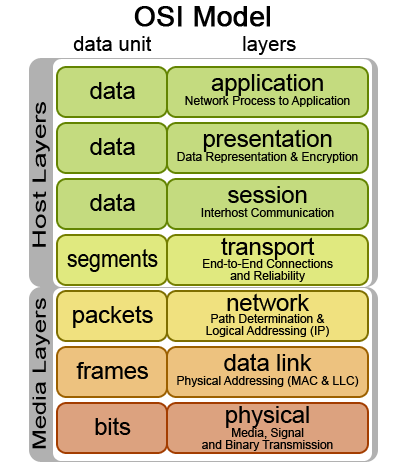
\includegraphics[width=5cm,height=5cm,keepaspectratio]{Images/OSIModel.png}
        \caption{OSI Model \cite{OSIPic}}
        \label{fig:OSIModel}
    \end{center}
\end{figure}

Network switches and network routers interpret the destination based off information found in
Layer 2 or Layer 3 from the OSI model, hence I must adhere to the protocol standards found at these
layers. Layers 4 and above provide other benefits to the payload such as reliability and is not a
concern for this project.

\subsection{Layer 1}

In Ethernet systems, Layer 1 refers to the physical medium that information is being sent over.
Gigabit ethernet based systems use a copper wire as the physical medium, with electrical voltages
representing the information. For this project, the latency is measured at this layer.

\subsection{Layer 2}

Layer 2 is responsible for transferring data between adjacent network devices \cite{IEEE802}. This is important as
information will be flowing to and from adjacent nodes, through a switch or router. To ensure that
information flows through the switch or router, this layer must be taken into consideration to ensure
successful transmission and reception of information.

\subsection{Layer 3}

Information from one hop to another is determined by the Layer 3 protocol. This ensures that
information is correctly routed to the destination from the source. This layer is important as the
information stored at this layer ensures the correct path is taken from sender to receiver. This is
different to Layer 2, as this can incorporate non-adjacent nodes as well.

\section{Latency Definitions}

Latency in a network can be defined in many of the following ways. These are important to the project as it will be focusing on One Way Trip time, because it is a subset of the other latencies.

\subsection{Connection Time}

Connection time is the time that two devices take to enable information flow between them. In
some cases, there are many synchronisation and authentication steps that need to take place before
any information can flow. This latency is defined as the initialization of the first command, to the
processing of the final command.

\subsection{Return Trip Time}

In some cases, the return trip time can be used to measure the one-way latency of two devices. One
device sends a request for an echo and when received, the time taken from transmit to receive is
twice the latency between devices.

\subsection{One way Trip Time}

Similar to Return Trip Time but instead of requiring an echo back to the sender, the receiver is on the
same device. Hence the latency of the connection is measured as the time taken for the information
to flow from one port on the device to another.

\section{Current Solutions}

\subsection{Ping}

Ping is a Linux utility that can be used to estimate the latency to a given network server. 
This is for large distance measurements, as the accuracy of this ranges from seconds to milliseconds. 
It has also been tested that this utility is unreliable for performance extensive testing as momentary ‘glitches’ can appear in networks, causing random and unpredictable results \cite{pingisbad}.
This does not meet the need of having the ability to measure time in the nanosecond range.

\subsection{Data plane Development Kit (DPDK)}

DPDK is a software implementation of rapid packet processing. 
This software utilises low level software drivers to interact directly with the hardware. 
Doing so requires specific hardware on the computer which needs to be compatible with the software itself.
Reducing the packet processing time reduces the time offset created by the CPU, but not fully removes it. 
Examples in the source code have shown that the timing value is dependent on CPU frequencies \cite{dpdkcode} and Dynamic Frequency scaling \cite{turboboost} of modern CPUs can cause a change in this frequency at any time.

\subsection{PF\textunderscore RING}

Another software solution is PF\textunderscore RING by ntop\texttrademark. 
It is a rapid packet processing library that does not require the need for specific hardware.  
PF\textunderscore RING allows for more efficient packet capturing and filtering by utilising more cores and threads on a CPU \cite{pfringworks}.
This library is more focused on throughput of packets processed rather than latency. 
This is less accurate than the DPDK but increases the flexibility of the platform it can implemented on. 
As with all software based approaches, this does not meet the requirements of being able to measure time in nanoseconds reliably.

\subsection{Data Acquisition and Generation (DAG) 10x2-S}

The DAG 10x2-S by Endace is a hardware based packet capturing solution with high precision nanosecond scale precision \cite{dagprecision}. 
This is a physical device which connects to a x86 based computer and communicates via Peripheral Component Interconnect Express (PCIe). 
The DAG 10x2-S is recommended for capturing network packets over gigabit ethernet links, as the other models cost more and have other unnecessary features \cite{dagfeatures}.
It is an expansion card for a computer which extends the capabilities of the computer to accurately capture and timestamp packets to a high degree. 
This device has the capabilities to timestamp packets with a resolution of 4ns \cite{dagprecision}. 
This meets all the requirements of the project but is very costly (\$2500 USD \cite{dagprice}) and methods for obtaining a device can only be done through Endace themselves. 

\section{Field Programmable Gate Array (FPGA)}

A FPGA is an array of configurable logic gates. The number of gates are in the order of thousands to
millions. This many configurable gates allows for complex logical structures and digital circuits to be
implemented in hardware, while consuming little physical space. This differs from a CPU, where the
logical gate circuitry is fixed, and manipulation of electrical Input/output must be done by clocking
through an instruction set. Without the need for an instruction set, FPGAs allow for high speed time
critical applications to be implemented without the overhead of needing to clock through CPU
instructions. This is important characteristic as the electrical signals measured from the network
interfaces are time critical.

\subsection{Xilinx Zynq FPGA}

Xilinx is a manufacturer of FPGAs, and a family of products they produce is the Zynq-7000 range \cite{fpga}.
These FPGAs integrate a dual-core ARM Cortex-A9 MPCore with FPGA gate fabric enabling high performance applications to run on the FPGA, while embedded programs can run on the ARM cores.
This project incorporates the FPGA section to manage the timing functions and the ARM section to run the application for storing the timing information.
